 \documentclass[journal,12pt,twocolumn]{IEEEtran}
%
\usepackage{setspace}
\usepackage{gensymb}
\singlespacing
\usepackage[cmex10]{amsmath}
\usepackage{amsthm}
\usepackage{mathrsfs}
\usepackage{txfonts}
\usepackage{stfloats}
\usepackage{bm}
\usepackage{cite}
\usepackage{cases}
\usepackage{subfig}
\usepackage{longtable}
\usepackage{multirow}
%\usepackage{algorithm}
\usepackage{enumitem}
\usepackage{mathtools}
\usepackage{steinmetz}
\usepackage{tikz}
\usepackage{circuitikz}
\usepackage{verbatim}
\usepackage{tfrupee}
\usepackage[breaklinks=true]{hyperref}
%\usepackage{stmaryrd}
\usepackage{tkz-euclide} % loads  TikZ and tkz-base
%\usetkzobj{all}
\usetikzlibrary{calc,math}
\usepackage{listings}
    \usepackage{color}                                            %%
    \usepackage{array}                                            %%
    \usepackage{longtable}                                        %%
    \usepackage{calc}                                             %%
    \usepackage{multirow}                                         %%
    \usepackage{hhline}                                           %%
    \usepackage{ifthen}                                           %%
  %optionally (for landscape tables embedded in another document): %%
    \usepackage{lscape}     
\usepackage{multicol}
\usepackage{chngcntr}
%\usepackage{enumerate}

%\usepackage{wasysym}
%\newcounter{MYtempeqncnt}
\DeclareMathOperator*{\Res}{Res}
%\renewcommand{\baselinestretch}{2}
\renewcommand\thesection{\arabic{section}}
\renewcommand\thesubsection{\thesection.\arabic{subsection}}
\renewcommand\thesubsubsection{\thesubsection.\arabic{subsubsection}}
\newcommand\numberthis{\addtocounter{equation}{1}\tag{\theequation}}
\renewcommand\thesectiondis{\arabic{section}}
\renewcommand\thesubsectiondis{\thesectiondis.\arabic{subsection}}
\renewcommand\thesubsubsectiondis{\thesubsectiondis.\arabic{subsubsection}}

% correct bad hyphenation here
\hyphenation{op-tical net-works semi-conduc-tor}
\def\inputGnumericTable{}                                 %%

\lstset{
%language=C,
frame=single, 
breaklines=true,
columns=fullflexible
}


\begin{document}
%


\newtheorem{theorem}{Theorem}[section]
\newtheorem{problem}{Problem}
\newtheorem{proposition}{Proposition}[section]
\newtheorem{lemma}{Lemma}[section]
\newtheorem{corollary}[theorem]{Corollary}
\newtheorem{example}{Example}[section]
\newtheorem{definition}[problem]{Definition}

\newcommand{\BEQA}{\begin{eqnarray}}
\newcommand{\EEQA}{\end{eqnarray}}
\newcommand{\define}{\stackrel{\triangle}{=}}
\bibliographystyle{IEEEtran}
%\bibliographystyle{ieeetr}
\providecommand{\mbf}{\mathbf}
\providecommand{\pr}[1]{\ensuremath{\Pr\left(#1\right)}}
\providecommand{\qfunc}[1]{\ensuremath{Q\left(#1\right)}}
\providecommand{\sbrak}[1]{\ensuremath{{}\left[#1\right]}}
\providecommand{\lsbrak}[1]{\ensuremath{{}\left[#1\right.}}
\providecommand{\rsbrak}[1]{\ensuremath{{}\left.#1\right]}}
\providecommand{\brak}[1]{\ensuremath{\left(#1\right)}}
\providecommand{\lbrak}[1]{\ensuremath{\left(#1\right.}}
\providecommand{\rbrak}[1]{\ensuremath{\left.#1\right)}}
\providecommand{\cbrak}[1]{\ensuremath{\left\{#1\right\}}}
\providecommand{\lcbrak}[1]{\ensuremath{\left\{#1\right.}}
\providecommand{\rcbrak}[1]{\ensuremath{\left.#1\right\}}}
\theoremstyle{remark}
\newtheorem{rem}{Remark}
\newcommand{\sgn}{\mathop{\mathrm{sgn}}}
\providecommand{\abs}[1]{\left\vert#1\right\vert}
\providecommand{\res}[1]{\Res\displaylimits_{#1}} 
\providecommand{\norm}[1]{\left\lVert#1\right\rVert}
%\providecommand{\norm}[1]{\lVert#1\rVert}
\providecommand{\mtx}[1]{\mathbf{#1}}
\providecommand{\mean}[1]{E\left[ #1 \right]}
\providecommand{\fourier}{\overset{\mathcal{F}}{ \rightleftharpoons}}
%\providecommand{\hilbert}{\overset{\mathcal{H}}{ \rightleftharpoons}}
\providecommand{\system}{\overset{\mathcal{H}}{ \longleftrightarrow}}
	%\newcommand{\solution}[2]{\textbf{Solution:}{#1}}
\newcommand{\solution}{\noindent \textbf{Solution: }}
\newcommand{\cosec}{\,\text{cosec}\,}
\providecommand{\dec}[2]{\ensuremath{\overset{#1}{\underset{#2}{\gtrless}}}}
\newcommand{\myvec}[1]{\ensuremath{\begin{pmatrix}#1\end{pmatrix}}}
\newcommand{\mydet}[1]{\ensuremath{\begin{vmatrix}#1\end{vmatrix}}}
\numberwithin{equation}{subsection}
\makeatletter
\@addtoreset{figure}{problem}
\makeatother
\let\StandardTheFigure\thefigure
\let\vec\mathbf
\renewcommand{\thefigure}{\theproblem}
\def\putbox#1#2#3{\makebox[0in][l]{\makebox[#1][l]{}\raisebox{\baselineskip}[0in][0in]{\raisebox{#2}[0in][0in]{#3}}}}
     \def\rightbox#1{\makebox[0in][r]{#1}}
     \def\centbox#1{\makebox[0in]{#1}}
     \def\topbox#1{\raisebox{-\baselineskip}[0in][0in]{#1}}
     \def\midbox#1{\raisebox{-0.5\baselineskip}[0in][0in]{#1}}
\vspace{3cm}
\title{Matrix Theory Assignment 1}
\author{Ritesh Kumar}

\maketitle
\newpage
%\tableofcontents
\bigskip
\renewcommand{\thefigure}{\theenumi}
\renewcommand{\thetable}{\theenumi}
\counterwithout{figure}{section}
\counterwithout{figure}{subsection}
%\begin{document}	
	%	\begin{titlepage}
%	\begin{center}
%		\vspace*{1cm}
%		
%		\textbf{ \huge{Assignment 1}}
%		\vspace{1.5cm}
%		
%		\textbf{Ritesh Kumar} \\
%		\textbf{(EE20RESCH11005)}\\
%		\textbf{Communication and Signal Processing}
		\date{Today}
		
%	\end{center}
	%	\end{titlepage}
	\begin{abstract}
		This document demonstrates a method to find the distance of a point from a line. And that point is along a line.
		\end{abstract}	
		Download all  codes from 
		
		\begin{lstlisting}
		https://github.com/Ritesh622/Assignment1
		\end{lstlisting}	
	\section{Problem Statement} 	




	Find the distance of the line 
	
	
	\begin{align}
\myvec{4 & 7}\myvec{X} = - 5 
\end{align}
from the point
$ \myvec
{				
1 \\
2 \\			
} $  along the line 
	\begin{align}
	\myvec{2 & -1}\myvec{X} = 0
	\end{align}
\section{solution}

\subsection {Finding the point of intersection using  row-echelon form}	

\begin{flushleft}
	We need to find the solution of equations:
	\begin{align}
	\myvec{4 & 7}\textbf{x} = - 5 \label{eqn1} \\
	\myvec{2 & - 1}\textbf{x} = 0\label{eqn2}
	\end{align}
	Transforming the matrix into row-echelon form \\
	\begin{align}
	\myvec{
		4 & 7 & -5 \\
		2 & 1 & 0\\
	}
	\xleftrightarrow[]{R1 \leftarrow \frac{1}{18}*(R1+ 7 \times R2) } \nonumber \label{eqn4} \\
	\myvec{
		1 & 0 & -5/18 \\
		2 & -1 & 0
	}
	\end{align}
	\begin{align}
	\myvec{
		1 & 0 & -5/18 \\
		2 & -1 & 0
	}
	\xleftrightarrow[]{R2 \leftarrow  -(R2- 2 \times R1) } \nonumber \label{eqn5}  \\
	\myvec{
		1 & 0 & -5/18 \\
		0 & 1 & -10/18
	}
	\end{align}
\end{flushleft}




\begin{figure}[htb!]	
	\centering	
	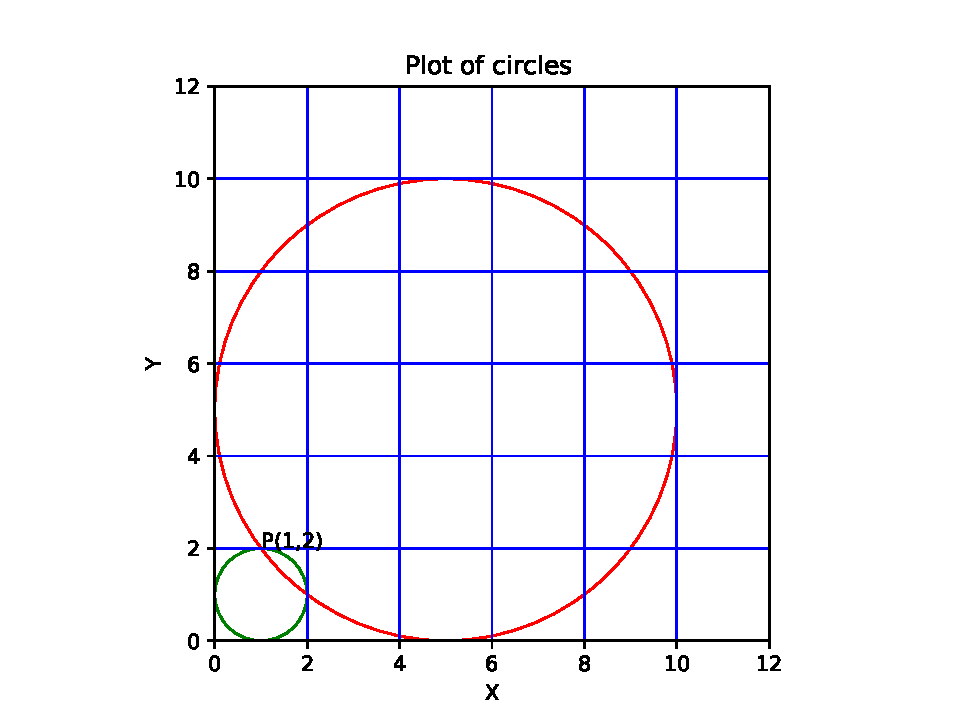
\includegraphics[width=.50\textwidth, height=.30\textheight]{Figure.pdf}	
	\caption{Intersection of two lines}
	\label{fig1}	
\end{figure}


After solving this two equation we will get the  point of intersection, which is intersection of these two lines segments.
Thus, point of intersection is $\myvec {-5/18 \\ -10/18 \\ } $.
Now we have point of intersection
\begin{align}
 \vec{P} = 
\myvec{
-5/18\\
-10/18 \\	
}
\end{align}
and given point is
\begin{align}
\vec{Q}   = 
\myvec
{
1\\
2 \\	
} 
\end{align}
Now  the distance between two points is given as :
\begin{align}
\norm{
\vec{P} - \vec{Q}
} = 
\norm {
\myvec{
-5/18\\ 
-10/18 \\
}
-  \myvec {
1\\ 
2 \\
} }= d = 2.85 
\end{align}

\end{document}
